\section{Injections}
\label{sec:appendix_injections}

This chapter describes some extra options when using our injections to integrate handwritten code with generated code. 
This complements the short introduction in Chapter~\ref{sec:intro_injections}.

As an example, we shall provide functionality for saving our \textsf{DoubleLinkedList} to a file.

\begin{enumerate}
  \item[$\blacktriangleright$] Begin with an empty workspace, create a new metamodel \textsf{Demo} and replace the \textsf{Demo.eap} with the file from our .zip file (in the folder containing this tutorial). 
  \item[$\blacktriangleright$] Now open \textsf{Demo.eap} and change the ``Default Language for Code Generation'' (Tools $\rightarrow$ Options $\rightarrow$ Source Code Engineering) to \textsf{Ecore}. 
  \item[$\blacktriangleright$] Add the method \textsf{void toFile(EString path)} to the class \textsf{List} (Fig.~\ref{fig:append_inj_diagram}) and export the project to your Eclipse workspace.
\end{enumerate}
\begin{figure}[htbp]
\begin{center}
  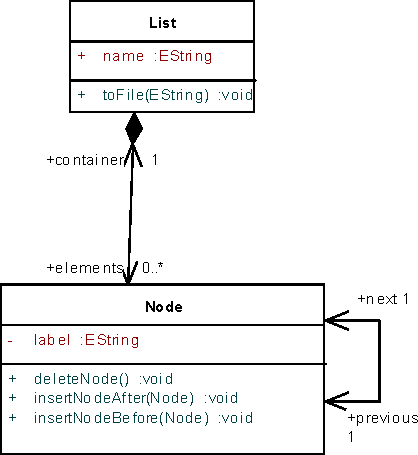
\includegraphics[width=0.5\textwidth]{pics/advancedTopics/injections/ea_diagram}
  \caption{Add a new method \textsf{toFile} to the class \textsf{List}}
  \label{fig:append_inj_diagram}
\end{center}
\end{figure}

\begin{enumerate}
  \item[$\blacktriangleright$] To implement the \textsf{toFile} method, right-click \textsf{gen/Double\-Linked\-List\-Language/\-List.java} in the generated Eclipse project and choose ``eMoflon/create Injection for class'', which will generate the file \textsf{injection/DoubleLinkedListLanguage/List.inject}.
	Insert the code depicted in Fig.~\ref{code:list_toFile_impl} into this file.
  \item[$\blacktriangleright$] To make use of some basic templates for code completion, type ``$@$'', press ``Ctrl+Shift'' and choose (in this case) ``Inject method in model''. 
  Functions that are annotated with \texttt{@model} implement methods that are defined in the interface of the model, i.e., are explicitly modelled as operations in EA, and have the structure:\\ 
  \texttt{@model [signature] <-- [code] -->}.
\end{enumerate}
\begin{figure}[htbp]
\centering
	\begin{lstlisting}[language=Injection]
	partial class List
	{
    	@model toFile(String path) <--

        	try{
            	FileWriter fstream = new FileWriter(path);
            	BufferedWriter out = new BufferedWriter(fstream);
            	out.write(this.toText());

            	out.close();
        	}catch (Exception e){
            	System.err.println(e.toString);
        	}

    	-->
	}
\end{lstlisting}
\caption{Injection for \textsf{List::toFile(String)}}
\label{code:list_toFile_impl}
\end{figure}

You may have noticed that we use an undefined method \textsf{List::toText()} in the implementation of the \textsf{toFile} method. 
We will now inject this as a private method in the implementation class \textsf{ListImpl.java}.

\begin{enumerate}
  \item[$\blacktriangleright$] Right-click \textsf{gen/DoubleLinkedListLanguage/impl/ListImpl.java} and choose ``eMoflon/create Injection for class'' to create \textsf{injection/DoubleLinkedListLanguage/impl/ListImpl.inject}.
  Implement the private method \textsf{toText()} with the code depicted in Fig.~\ref{code:listImpl_toText_impl}.  
  \item[$\blacktriangleright$] When you now rebuild the project (right-click on \textsf{DoubleLinkedListLanguage} and choose ``eMoflon/Build and Clean''), this code will be injected into \textsf{ListImpl.java}. 
\end{enumerate}
 
\begin{figure}[htbp]
\centering
\begin{lstlisting}[language=Injection]
import java.io.*;

partial class ListImpl
{
    @members <--

    private String toText(){
        StringBuilder sb = new StringBuilder();

        for(Node element : elements){
            sb.append(element.getLabel());
            sb.append("\n");
        }

        return sb.toString();
    }

    -->
}
\end{lstlisting}
\caption{Injection for \textsf{toText()} in \textsf{ListImpl.java}}
\label{code:listImpl_toText_impl}
\end{figure}

In this way, member functions and fields that were \emph{not} modelled in EA can be injected using the \texttt{@members} keyword. 
Everything between \texttt{<--  -->} is copied into the end of the generated \textsf{ListImpl.java} file without any restrictions at all.
Note how imports can also be injected (as done here for \textsf{java.io.*}). 

Although it is possible to inject members in the interface file (i.e., \textsf{List.java} in this example), this is considered dirty and should be used very sparingly (if possible never). 
You can have several \texttt{@model} injections in your \textsf{.inject} file, but only a single \texttt{@member} scope.

\clearpage